% Chapter Template

\chapter{Desarrollo}

\label{Chapter4} % Change X to a consecutive number; for referencing this chapter elsewhere, use \ref{ChapterX}

Una vez presentado el contexto, en este capítulo se detallará la solución software final desarrollada. En primer lugar se presenta el diseño realizado con cada una de sus partes y el desarrollo total en cada una de sus partes. MEJORAR!!!


%-----------------------------------
%	SECTION Diseño
%-----------------------------------
\section{Diseño}

El trabajo se basa principalmente en dos componentes; un componente de JDeRobot (\textbf{OpenniServer}) que funciona como driver del sensor y proporciona las imágenes recogidas por éste y el componente realizado (\textbf{realRTEstimator}) que se encargará, una vez recogidas las imágenes, de toda la lógica restante.

El objetivo del componente consiste en analizar en tiempo real la posición y movimiento del sensor, por lo que el componente deberá dar una estimación en todo momento.

En la Figura~\ref{fig:diagram1} se puede apreciar el diagrama global de funcionamiento del componente desarrollado y su conexión con los otros componentes y los diferentes datos de entrada. OpenniServer se encarga de preparar y enviar las imágenes del sensor al componente que es el encargado de procesarlas. El componente también recibe los datos de los parámetros intrínsecos de la cámara. A su salida el componente entregará una matriz RT que describe la posición y orientación absolutas en ese preciso instante de tiempo. 

\begin{figure}[th]
\centering
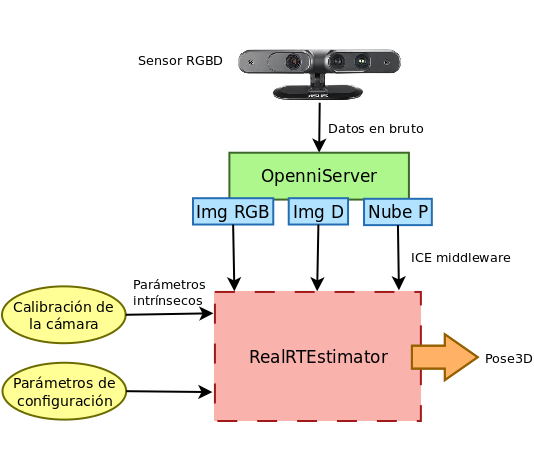
\includegraphics[scale=0.42]{Figures/diagram1.png}
\decoRule
\caption[Diagram1]{Esquema global de funcionamiento.}
\label{fig:diagram1}
\end{figure}


\begin{figure}[th]
\centering
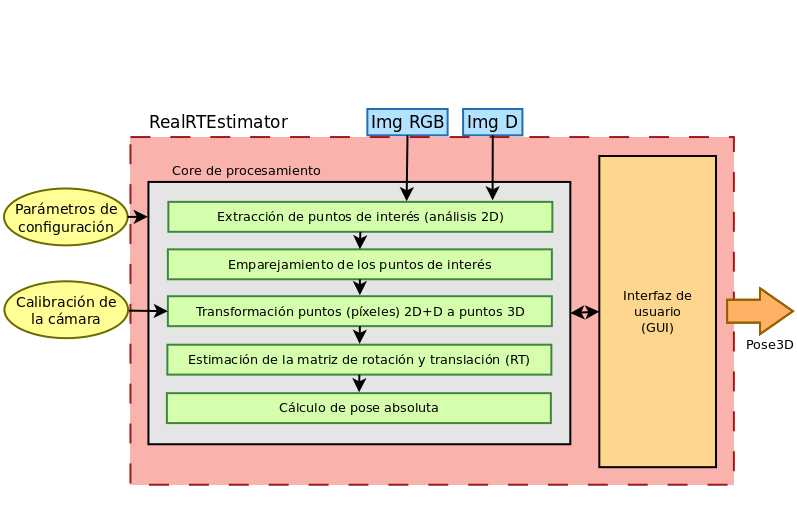
\includegraphics[scale=0.35]{Figures/diagram2.png}
\decoRule
\caption[Diagram2]{Diagrama del componente RealRTEstimator.}
\label{fig:diagram2}
\end{figure}

%-----------------------------------
%	SECTION Extracción de características de una imágen
%-----------------------------------
\section{Análisis 2D}

Extracción de características de una imágen

\subsection{Puntos de interés}

%-----------------------------------
%	SECTION Emparejamiento (\textit{matching})
%-----------------------------------
\section{Emparejamiento (\textit{matching})}

%-----------------------------------
%	SUBSECTION Cálculo de movimiento
%-----------------------------------
\section{Cálculo de movimiento}

\subsection{Matriz RT}

%-----------------------------------
%	SECTION Interfaz gráfica
%-----------------------------------
\section{Interfaz gráfica}